\chapter{Melhores práticas de planejamento de TI relacionadas ao problema do PDTI}
\label{capitulo:proposta_mp}

O foco desta pesquisa consiste em esclarecer as razões que culminam no problema de planejamento de TI das instituições públicas federais. A metodologia adotada nesta pesquisa permitiu expor os fatores que atrapalham as instituições a elaborarem o PDTI, na visão dos participantes desta atividade. Apesar destes elementos comporem o objetivo principal da presente pesquisa, propõe-se além disso, sugerir um conjunto de melhores práticas para atenuar os fatores que restringem a elaboração e a qualidade do PDTI.

As práticas propostas neste capítulo são inteiramente baseadas na tese de \citeonline{teixeira:10}. O autor propõe um modelo de maturidade para planejamento estratégico de SI/TI direcionado às organizações governamentais brasileiras (MMPE-SI/TI Gov) baseado em melhores práticas. O método \textit{Grounded Theory} também foi empregado nesta etapa da pesquisa com o intuito de prover rigor científico à seleção das melhores práticas que atingem diretamente os fatores causais presentes nas teorias resultantes.
%Diante do banco de melhores práticas proposto por \citeonline{teixeira:10}, foi feito o mapeamento daquelas que atingem diretamente os fatores presentes nas teorias resultantes desta pesquisa.


\section{Processos e Melhores Práticas de Planejamento de TI}
\label{secao:melhores_praticas}
``Melhores práticas (MP) são visões de organizações e profissionais globais que através da vivência no mercado conseguem perceber práticas, que se utilizadas em outras organizações podem melhorar seu desempenho da mesma forma'' \apud{kerzner:11,laudon:05}{teixeira:10}.

O modelo de maturidade MMPE-SI/TI (Gov) foi definido em conformidade com os principais modelos e normas nacionais e internacionais utilizados para definição e avaliação de processos, tais como ISO 12207/15504, COBIT, CMMI, MPS.BR, MMGP, OPM3, PMMM, leis e normativas do governo brasileiro. Sua estrutura é composta por um modelo de referência (MR), um método de avaliação (MA) e um banco de melhores práticas (BMP). 

O modelo MMPE-SI/TI (Gov) possui 5 níveis de maturidade, 6 níveis de capacidade, 16 processos e 124 melhores práticas para planejamento estratégico de SI/TI direcionadas às organizações governamentais brasileiras. A Tabela \ref{tabela:niveis_maturidade} apresenta os níveis de maturidade do modelo e seus processos.

\begin{table}[]
\centering
\begin{tabular}{|c|l|l|}
\hline
\rowcolor[HTML]{C0C0C0} 
\textbf{Nível} & \multicolumn{1}{c|}{\cellcolor[HTML]{C0C0C0}\textbf{Processos}}                                                                                                                                                                                & \multicolumn{1}{c|}{\cellcolor[HTML]{C0C0C0}\textbf{Áreas}}                                           \\ \hline
1 Inicial / ad hoc             & \begin{tabular}[c]{@{}l@{}}Promover Consciência Estratégica (PCE)\\ Assegurar Conformidade Governamental (ACG)\end{tabular}                                                                                                                    & \begin{tabular}[c]{@{}l@{}}Gestão\\ Organização\end{tabular}                                          \\ \hline
2 Gerenciado             & \begin{tabular}[c]{@{}l@{}}Gerenciar Recursos Humanos (GRH) \\ Educar e Treinar Pessoas (ETP) \\ Gerenciar Projetos (GEP) \\ Gerenciar Medição e Análise (GMA)\end{tabular}                                                                    & \begin{tabular}[c]{@{}l@{}}Pessoas\\ Pessoas\\ Gestão\\ Gestão\end{tabular}                           \\ \hline
3 Definido             & \begin{tabular}[c]{@{}l@{}}Definir o Processo Organizacional (DPO)\\ Gerenciar Aquisições e Terceirizações (GAT) \\ Gerenciar Infraestrutura de SI/TI (GIN) \\ Gerenciar Qualidade (GQA) \\ Fomentar Gestão do Conhecimento (FGC)\end{tabular} & \begin{tabular}[c]{@{}l@{}}Organização\\ Organização\\ Tecnologia\\ Gestão\\ Organização\end{tabular} \\ \hline
4 Medido             & \begin{tabular}[c]{@{}l@{}}Avaliar o Processo Organizacional (APO) \\ Gerenciar Riscos (GRI) \\ Gerenciar Integração com o Cidadão (GIC)\end{tabular}                                                                                          & \begin{tabular}[c]{@{}l@{}}Organização\\ Gestão\\ Pessoas\end{tabular}                                \\ \hline
5 Otimizado             & \begin{tabular}[c]{@{}l@{}}Melhorar o Processo Organizacional (MPO)\\  Otimizar a Gestão Organizacional (OGO)\end{tabular}                                                                                                                     & \begin{tabular}[c]{@{}l@{}}Organização\\ Gestão\end{tabular}                                          \\ \hline
\end{tabular}
\caption{Níveis de Maturidade do MMPE-SI/TI (Gov) e seus Processos, extraído de \cite{teixeira:10}}
\label{tabela:niveis_maturidade}
\end{table}

Cada processo contém um conjunto de melhores práticas (MP) e resultados esperados (RE). A seleção das MP aderentes aos cenários levantados nesta pesquisa - em relação ao problema do planejamento de TI - tem o intuito de sugerir um caminho para atenuar os efeitos das condições causais e dos fenômenos centrais das teorias que emergiram dos dados. O procedimento realizado para selecionar as MP relacionadas com as duas teorias fundamentadas nos dados desta pesquisa é descrito na seção seguinte.

%Ao traçar relações entre MP, condições causais e os fenômenos centrais, busca-se oferecer meios para reduzir as consequências (problemas na elaboração do planejamento de TI). Este objetivo foi possível investigando possíveis relações entre os processos do MMPE-SI/TI e os elementos das teorias que emergiram dos dados nesta pesquisa. Este procedimento é descrito na seção seguinte. 
%Diante do exposto, o objetivo secundário desta pesquisa se propõe a realizar uma seleção das melhores práticas de planejamento estratégico de SI/TI direcionadas aos fatores que restringem o planejamento de TI nas instituições pesquisadas.
\section{Seleção das Melhores Práticas}

Para manter a coerência de fundamentação dos resultados desta pesquisa, optou-se por utilizar o mesmo método usado para gerar as teorias também na etapa de seleção das melhores práticas. A \textit{Grounded Theory} é aplicada neste contexto com o intuito de manter a fidelidade empírica que a teoria fundamentada nos dados carrega ao relacioná-la com processos e melhores práticas de planejamento de TI. Desta forma, a arbitrariedade do pesquisador ao selecionar as MP é reduzida e o grau de fundamentação nos dados é maximizado.

Buscou-se por relacionamentos entre elementos das teorias apresentadas nesta pesquisa e processos do MMPE-SI/TI (Gov) que, por sua vez, carregam seus respectivos conjuntos de MP. Assim, o esforço nesta etapa da pesquisa concentra-se em descobrir as relações semânticas entre as teorias fundamentadas nos dados e os processos de planejamento de TI do modelo de maturidade estudado. As melhores práticas já foram relacionadas aos processos no trabalho de \citeonline{teixeira:10} e serão apontadas como consequência do relacionamento com os processos. A Figura \ref{figura:esquemaconjuntos} representa graficamente esta ideia, onde as setas pontilhadas são os relacionamentos que se deseja descobrir.

\begin{figure}[h!]
\centering % para centralizarmos a figura
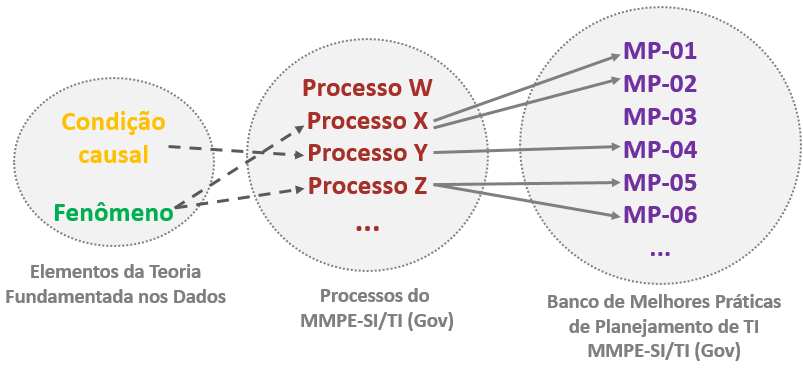
\includegraphics[width=13cm]{figuras/conjuntos_relacionamentos.PNG}
\caption{Esquema de relacionamento entre elementos da teoria e processos de planejamento.}
\label{figura:esquemaconjuntos}
\end{figure}

Para focar a busca por processos diretamente relacionados aos elementos centrais das teorias, as mesmas foram reescritas na forma de paradigma, conforme descreve \citeonline{corbin:98}. Abaixo, cada uma das teorias com seus respectivos elementos organizados de acordo com o paradigma causal:
\\
\\
\textbf{Teoria 1:}\\
\textit{Condição causal:} Nível baixo de maturidade em gestão;\\
\textit{Fenômeno:} Deficiências estratégicas na TI;\\
\textit{Consequência:} Ausência de planejamento de TI.
\\
\\
\textbf{Teoria 2:}\\
\textit{Condição causal:} A tríade ``problemas de cultura organizacional'' + ``TI não reconhecida estrategicamente'' + ``problemas com recursos humanos'';\\
\textit{Fenômeno:} Problemas na participação das áreas de negócio;\\
\textit{Consequência:} Dificuldades na elaboração do planejamento e PDTI com deficiências.

De posse dos elementos de cada teoria e dos processos do modelo MMPE-SI/TI (Gov), aplicou-se a \textit{Grounded Theory} para traçar as relações entre estes dois grupos de dados. Como não há nesta fase o objetivo de gerar uma nova teoria ou eleger uma categoria central, aplicou-se apenas as etapas de codificação aberta e axial.

\subsection{Codificação Aberta}

Diferentemente da primeira etapa desta pesquisa, onde foi necessário identificar os códigos nos dados coletados através dos questionários, nesta segunda aplicação do método GT aproveitou-se os códigos (categorias) da primeira etapa. Porém, para relacionar as categorias da teoria existente aos processos do MMPE-SI/TI, se faz necessário codificá-los.

Cada processo do MMPE-SI/TI foi codificado como uma categoria, rotulada com o mesmo nome do processo. O a descrição da categoria é o próprio propósito do processo descrito por \citeonline{teixeira:10}. Os resultados esperados de cada processo definem os mesmos, ou seja, o conjunto de RE de cada processo podem ser considerados como propriedades das categorias. Abaixo é apresentado um exemplo da codificação aberta de um dos processos. A Tabela \ref{tabela:mmpe_to_gt} mostra os dados extraídos do MMPE-SI/TI e os itens correspondentes na codificação aberta.

%PAREI AQUI: fazer tabela
% Please add the following required packages to your document preamble:
% \usepackage[table,xcdraw]{xcolor}
% If you use beamer only pass "xcolor=table" option, i.e. \documentclass[xcolor=table]{beamer}
\begin{table}[]
\centering
\resizebox{\textwidth}{!}{%
\begin{tabular}{|l|l|}
\hline
\rowcolor[HTML]{C0C0C0} 
\multicolumn{1}{|c|}{\cellcolor[HTML]{C0C0C0}\textbf{MMPE-SI/TI (Gov)}}                                                                                                                                                                                                                                                                                       & \multicolumn{1}{c|}{\cellcolor[HTML]{C0C0C0}\textbf{Grounded Theory}}                                                                                                                                                                                                                                                                            \\ \hline
\textbf{Processo:} Educar e Treinar Pessoas (ETP)                                                                                                                                                                                                                                                                                                                      & \textbf{Categoria:} CAT Educar e Treinar Pessoas                                                                                                                                                                                                                                                                                                          \\ \hline
\begin{tabular}[c]{@{}l@{}}\textbf{Propósito:} Entender claramente as necessidades\\ das pessoas (diretores, gerentes e usuários) em \\ termos de educação e treinamento em SI/TI e \\ executar uma estratégia eficaz de treinamento \\ e medição dos resultados.\end{tabular}                                                                                         & \begin{tabular}[c]{@{}l@{}}\textbf{Conceito:} Entender claramente as necessidades\\ das pessoas (diretores, gerentes e usuários) em \\ termos de educação e treinamento em SI/TI e \\ executar uma estratégia eficaz de treinamento\\ e medição dos resultados.\end{tabular}                                                                              \\ \hline
\begin{tabular}[c]{@{}l@{}}\textbf{Resultados Esperados (RE):}\\ ETP-RE-01: Treinamentos para tratar das \\ necessidades da organização são desenvolvidos\\ ou adquiridos;\\ \\ ETP-RE-02: Treinamentos para garantir que \\ todos os indivíduos têm habilidades necessárias \\ para executar as suas tarefas são realizados, \\ monitorados e avaliados.\end{tabular} & \begin{tabular}[c]{@{}l@{}}\textbf{Propriedades:}\\ ETP-RE-01: Treinamentos para tratar das \\ necessidades da organização são desenvolvidos\\ ou adquiridos;\\ \\ ETP-RE-02: Treinamentos para garantir que \\ todos os indivíduos têm habilidades necessárias \\ para executar as suas tarefas são realizados, \\ monitorados e avaliados.\end{tabular} \\ \hline
\end{tabular}%
}
\caption{Exemplo de categoria codificada a partir de um processo.}
\label{tabela:mmpe_to_gt}
\end{table}

O procedimento de codificar os processos em categorias foi realizado com os 16 processos do modelo de maturidade, portanto acrescentando 16 novas categorias ao conjunto de códigos de cada uma das duas teorias fundamentadas nos dados. O passo seguinte é pesquisar por relacionamentos entre as novas categorias e as categorias de cada teoria central, este procedimento é realizado na codificação axial.

\subsection{Codificação Axial}
A codificação axial tem por objetivo descobrir possíveis relações entre categorias. O procedimento para realizar esta codificação, assim como realizado para descobrir as teorias, consiste em colocar cada categoria como eixo e buscar relações semânticas com outras categorias \cite{glaser:68, corbin:98}.

Os conectores usados na codificação axial para descobrir as teorias foram: \textit{is a}, \textit{is cause of}, \textit{is part of} e \textit{is associated with}. Contudo, nesta etapa da pesquisa, estes conectores não são compatíveis com a semântica que a análise dos dados demonstrou. As categorias extraídas do modelo de maturidade apresentam um sentido de efeitos de uma solução, ao contrário das categorias das teorias que apresentam sentido de causas de problemas. 

Neste cenário, \citeonline{corbin:98} apresenta o tipo de relacionamento denominado ``condição interveniente''. A condição interveniente representa relacionamentos onde o código origem representa um conceito que pode reduzir ou alterar o impacto do código destino no fenômeno. Desta forma, é possível representar relações entre códigos que possuem sentido oposto um ao outro. Com isto, foi introduzido o conector \textit{contradicts} para representar as condições intervenientes.

A descoberta dos relacionamentos entre as teorias sobre os problemas de planejamento de TI e os processos do modelo de maturidade foi facilitada observando os resultados esperados de cada processo. Observa-se que os RE são opostos às propriedades das categorias da teoria. As análises apontam para a seguinte linha de pensamento: a instituição que apresenta estes fatores causais (do problema) não apresenta os resultados esperados deste processo. 

Para a teoria 1, das instituições que não possuem PDTI, a codificação axial permitiu trazer à tona 4 processos que impactam diretamente nas causas do problema: Promover Consciência Estratégica (PCE); Gerenciar Recursos Humanos (GRH); Educar e Treinar Pessoas (ETP); Gerenciar Projetos (GEP). A Figura \ref{figura:teoria_processos_grupo1} apresenta o esquema teórico dos elementos da teoria 1 e as categorias de processos que apresentaram pelo menos um relacionamento com a teoria.

\begin{figure}[h!]
\centering % para centralizarmos a figura
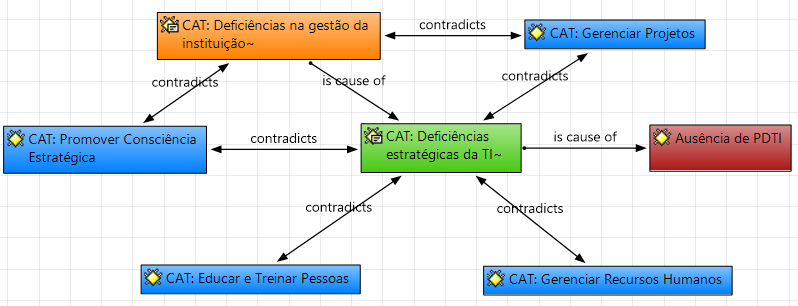
\includegraphics[width=15cm]{figuras/teoria_processos_grupo1.PNG}
\caption{Esquema teórico: Teoria 1 - Processos MMPE-SI/TI}
\label{figura:teoria_processos_grupo1}
\end{figure}

Para a teoria 2, das instituições que possuem PDTI, a codificação axial permitiu trazer à tona 5 processos que impactam diretamente nas causas do problema: Promover Consciência Estratégica (PCE); Gerenciar Recursos Humanos (GRH); Educar e Treinar Pessoas (ETP); Gerenciar Projetos (GEP); Otimizar a Gestão Organizacional (OGO). A Figura \ref{figura:teoria_processos_grupo2} apresenta o esquema teórico dos elementos da teoria 2 e as categorias de processos que apresentaram pelo menos um relacionamento com a teoria.

\begin{figure}[h!]
\centering % para centralizarmos a figura
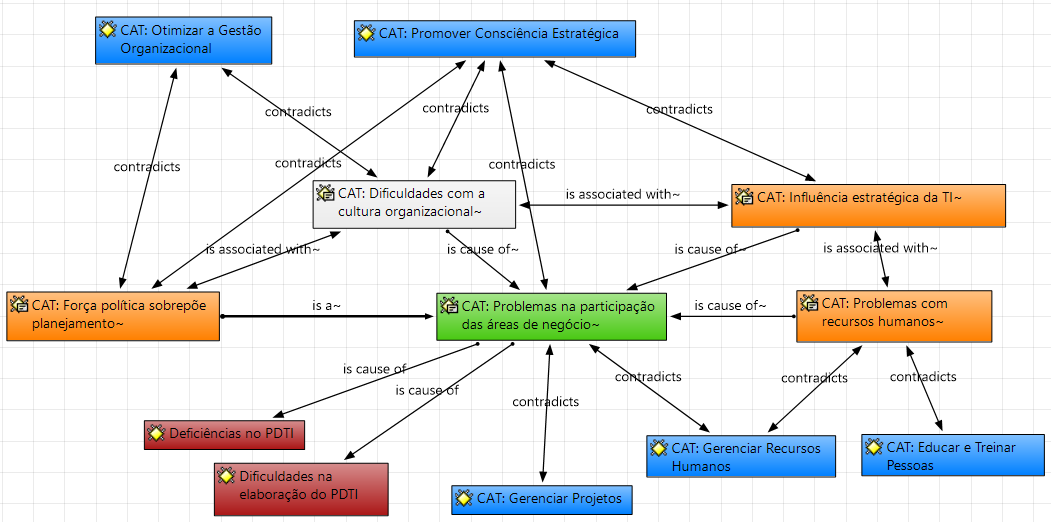
\includegraphics[width=15cm]{figuras/teoria_processos_grupo2.PNG}
\caption{Esquema teórico: Teoria 2 - Processos MMPE-SI/TI}
\label{figura:teoria_processos_grupo2}
\end{figure}

As análises foram registradas em notas de codificação axial e permitem compreender a relação semântica entre os códigos. De forma geral, foi observado que as relações eram descobertas analisando como o propósito e os resultados esperados do processo contrastavam com as categorias da teoria. Todas as notas de codificação axial desta etapa da pesquisa estão listadas no apêndice \autoref{apendice:j_notas_ac}.

É importante observar que o fenômeno central de ambas as teorias foi o elemento causal que concentrou mais relacionamentos com as categorias que representam os processos de planejamento de TI. Este efeito corrobora a conclusão de que as ``deficiências estratégicas da TI'' representam a principal causa da falta de PDTI (Teoria 1); e que os ``problemas na participação das áreas de negócio no planejamento de TI'' representam a principal causa das dificuldades de elaboração e deficiências no planejamento de TI das instituições que possuem PDTI.

\subsection{Melhores Práticas para Minimizar o Problema do PDTI}
\label{secao:mp_finais}

Ao aplicar as técnicas da \textit{Grounded Theory} foi possível vincular a teoria fundamentada nos dados que explica as causas dos problemas do PDTI nas instituições pesquisadas com os processos de planejamento de TI do MMPE-SI/TI (Gov). A Tabela \ref{tabela:processo_teoria} apresenta os processos de planejamento envolvidos diretamente com cada elemento causal das teorias.

\begin{table}[h!]
\centering
\resizebox{\textwidth}{!}{%
\begin{tabular}{c|l|l|}
\cline{2-3}
\textbf{}                                                                                                 & \multicolumn{1}{c|}{\cellcolor[HTML]{C0C0C0}\textbf{Elemento causal}}                                       & \multicolumn{1}{c|}{\cellcolor[HTML]{C0C0C0}\textbf{Processos envolvidos}}                                                                                                    \\ \hline
\multicolumn{1}{|c|}{\cellcolor[HTML]{C0C0C0}\textbf{\begin{tabular}[c]{@{}c@{}}Teoria\\ 1\end{tabular}}} & Deficiências na gestão da instituição                                                                       & \begin{tabular}[c]{@{}l@{}}PCE - Promover Consciência Estratégica\\ GEP - Gerenciar Projetos\end{tabular}                                                                     \\ \cline{2-3} 
\multicolumn{1}{|c|}{\cellcolor[HTML]{C0C0C0}\textbf{}}                                                   & Deficiências estratégicas na TI                                                                             & \begin{tabular}[c]{@{}l@{}}PCE - Promover Consciência Estratégica\\ GEP - Gerenciar Projetos\\ GRH - Gerenciar Recursos Humanos\\ ETP - Educar e Treinar Pessoas\end{tabular} \\ \hline
\multicolumn{1}{|c|}{\cellcolor[HTML]{C0C0C0}\textbf{\begin{tabular}[c]{@{}c@{}}Teoria\\ 2\end{tabular}}} & Problemas na cultura organizacional                                                                         & \begin{tabular}[c]{@{}l@{}}PCE - Promover Consciência Estratégica\\ OGO - Otimizar a Gestão Organizacional\end{tabular}                                                       \\ \cline{2-3} 
\multicolumn{1}{|c|}{\cellcolor[HTML]{C0C0C0}\textbf{}}                                                   & TI não reconhecida estrategicamente                                                                         & PCE - Promover Consciência Estratégica                                                                                                                                        \\ \cline{2-3} 
\multicolumn{1}{|c|}{\cellcolor[HTML]{C0C0C0}\textbf{}}                                                   & Problemas com recursos humanos                                                                              & \begin{tabular}[c]{@{}l@{}}GRH - Gerenciar Recursos Humanos\\ ETP - Educar e Treinar Pessoas\end{tabular}                                                                     \\ \cline{2-3} 
\multicolumn{1}{|c|}{\cellcolor[HTML]{C0C0C0}\textbf{}}                                                   & \begin{tabular}[c]{@{}l@{}}Problemas na participação das áreas\\ negócio no planejamento de TI\end{tabular} & \begin{tabular}[c]{@{}l@{}}PCE - Promover Consciência Estratégica\\ GRH - Gerenciar Recursos Humanos\\ GEP - Gerenciar Projetos\end{tabular}                                  \\ \hline
\end{tabular}%
}
\caption{Processos relacionados às teorias fundamentadas nos dados.}
\label{tabela:processo_teoria}
\end{table}

O propósito de cada um destes processos é descrito por \citeonline{teixeira:10} a seguir:

%Diante disso, foram mapeados um total de cinco processos que, se executados, podem contribuir para a melhoria da situação do planejamento de TI nas instituições públicas pesquisadas. O propósito de cada um destes processos é descrito por \citeonline{teixeira:10} a seguir:

\textbf{Promover Consciência Estratégica (PCE):} Habilitar a organização, através da alta administração, a entender as questões estratégicas de SI/TI, tais como os papéis de SI/TI, as capacidades e os conhecimentos tecnológicos, além de certificar-se de que há um entendimento comum entre o negócio e SI/TI, principalmente quanto ao potencial de contribuição que SI/TI proporciona para a estratégia do negócio.

%\textbf{Assegurar Conformidade Governamental (ACG):} Assegurar que a organização esteja em conformidade com os requisitos contratuais e legais (leis, decretos, instruções normativas, entre outras regulamentações) estabelecidas pelo governo brasileiro.

\textbf{Gerenciar Recursos Humanos (GRH):} Gerenciar os recursos humanos da organização e manter suas competências de acordo com as necessidades do negócio, além de motivar o pessoal de SI/TI através de planos de carreira, atribuição de funções coerentes com suas habilidades, definição de um processo de revisão do desempenho profissional, criação de descrições dos cargos, trabalho em grupo e minimização da dependência de indivíduos-chave.

\textbf{Educar e Treinar Pessoas (ETP):} Entender claramente as necessidades das pessoas (diretores, gerentes e usuários) em termos de educação e treinamento em SI/TI e executar uma estratégia eficaz de treinamento e medição dos resultados.

\textbf{Gerenciar Projetos (GEP):} Identificar, estabelecer, coordenar e monitorar as atividades, tarefas e recursos necessários para um projeto (planejamento de TI), com o objetivo de produzir um produto e/ou serviço, no contexto das necessidades do projeto e de suas restrições.

\textbf{Otimizar a Gestão Organizacional (OGO):} Otimizar e aperfeiçoar a gestão estratégica de SI/TI e as melhores práticas para planejamento estratégico de SI/TI da organização, buscando aumentar continuamente o alinhamento e a consistência com os objetivos estratégicos de negócio.


De acordo com o modelo de maturidade proposto por \citeonline{teixeira:10}, cada processo possui um conjunto de melhores práticas (MP). A seguir são apresentadas as 48 MP, propostas no MMPE-SI/TI (Gov), dos processos mapeados anteriormente.

\textbf{Melhores práticas do processo PCE: }
\\PCE-MP-01: Desenvolver uma Visão Estratégica; 
\\PCE-MP-02: Definir a Estrutura do Processo;
\\PCE-MP-03: Definir uma Estratégia;
\\PCE-MP-04: Consolidar o Compromisso com a Alta Administração;
\\PCE-MP-05: Comunicar a Visão e os Objetivos;
\\PCE-MP-06: Garantir o Compartilhamento de uma Visão Comum;
\\PCE-MP-07: Habilitar a Participação Ativa dos Stakeholders;
\\PCE-MP-08: Estabelecer um Comitê Estratégico de SI/TI (comitê de TI);
\\PCE-MP-09: Estabelecer um Plano Estratégico de SI/TI (ou PDTI).

\textbf{Melhores práticas do processo GRH: }
\\GRH-MP-01: Identificar Habilidades e Competências;
\\GRH-MP-02: Definir Critérios de Avaliação;
\\GRH-MP-03: Estabelecer um Programa de Recrutamento;
\\GRH-MP-04: Desenvolver Habilidades e Competências;
\\GRH-MP-05: Definir a Organização das Equipes;
\\GRH-MP-06: Conscientizar os Indivíduos sobre o Trabalho em Equipe;
\\GRH-MP-07: Manter as Interações das Equipes;
\\GRH-MP-08: Avaliar o Desempenho das Equipes;
\\GRH-MP-09: Fornecer Feedback sobre o Desempenho;
\\GRH-MP-10: Manter Registros de Pessoal;
\\GRH-MP-11: Minimizar a Dependência de Indivíduos-Chave;
\\GRH-MP-12: Organizar a Mudança e Desligamento do Cargo.

\textbf{Melhores práticas do processo ETP: }
\\ETP-MP-01: Desenvolver uma Estratégia de Treinamento;
\\ETP-MP-02: Identificar as Necessidades de Treinamento;
\\ETP-MP-03: Desenvolver ou Adquirir Treinamento;
\\ETP-MP-04: Preparar para Executar o Treinamento;
\\ETP-MP-05: Realizar o Treinamento do Pessoal;
\\ETP-MP-06: Manter os Registros de Treinamento;
\\ETP-MP-07: Avaliar a Eficácia do Treinamento.

\textbf{Melhores práticas do processo GEP: }
\\GEP-MP-01: Definir o Escopo do Projeto;
\\GEP-MP-02: Definir o Ciclo de Vida do Projeto;
\\GEP-MP-03: Avaliar a Viabilidade do Projeto;
\\GEP-MP-04: Determinar e Manter Estimativas para o Projeto;
\\GEP-MP-05: Definir as Atividades do Projeto;
\\GEP-MP-06: Definir as Necessidades de Experiências, Conhecimentos e Habilidades;
\\GEP-MP-07: Definir o Cronograma do Projeto;
\\GEP-MP-08: Identificar e Monitorar as Interfaces do Projeto;
\\GEP-MP-09: Atribuir Responsabilidades e Gerar Comprometimento;
\\GEP-MP-10: Estabelecer o Plano de Projeto;
\\GEP-MP-11: Implementar o Plano de Projeto;
\\GEP-MP-12: Monitorar o Projeto;
\\GEP-MP-13: Revisar o Progresso do Projeto;
\\GEP-MP-14: Corrigir os Desvios;
\\GEP-MP-15: Registrar Lições Aprendidas.

\textbf{Melhores práticas do processo OGO: }
\\OGO-MP-01: Priorizar Investimentos em Gestão Estratégica de SI/TI;
\\OGO-MP-02: Identificar Melhorias para Gestão Estratégica de SI/TI;
\\OGO-MP-03: Avaliar a Eficácia das Melhores Práticas;
\\OGO-MP-04: Aperfeiçoar as Melhores Práticas;
\\OGO-MP-05: Otimizar a Utilização das Melhores Práticas.


%
%Propõe-se, então, às instituições que enfrentam os problemas levantados nesta pesquisa que implementem os processos correspondentes ao cenário em que se encaixa. Em um primeiro cenário (grupo 1), instituições que ainda não possuem um PDTI e deseja minimizar os fatores que as impedem de elaborar o plano. O segundo cenário (grupo 2) engloba instituições que possuem um PDTI, mas que desejam minimizar as dificuldades na elaboração do plano. A Figura \ref{figura:processos_grupos} apresenta as camadas de processos que cada grupo precisa implementar. A ordem sugerida para implantação dos processos é da base para o topo da pirâmide.
%
%\begin{figure}[h!]
%\centering % para centralizarmos a figura
%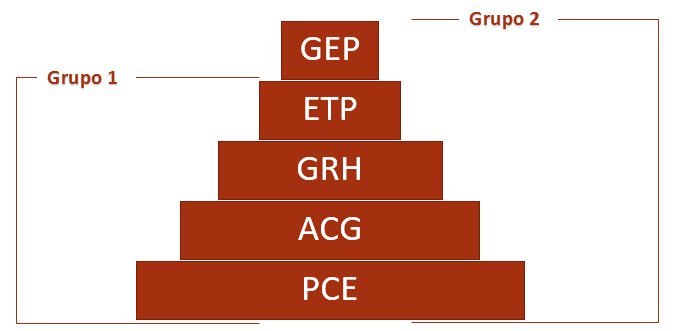
\includegraphics[width=8cm]{figuras/processos_grupos.PNG}
%\caption{Processos a serem implantados em cada cenário.}
%\label{figura:processos_grupos}
%\end{figure}

Tomando cada processo como eixo, as Tabelas \ref{tabela:acoes_1}, \ref{tabela:acoes_3}, \ref{tabela:acoes_4},  \ref{tabela:acoes_5} e \ref{tabela:acoes_2} apresentam as melhores de cada processo e seus respectivos resultados esperados.


\begin{table}[H]
\centering
\begin{tabular}{|l|l|}
\hline
\rowcolor[HTML]{C0C0C0} 
\multicolumn{1}{|c|}{\cellcolor[HTML]{C0C0C0}\textbf{MP}}                      & \multicolumn{1}{c|}{\cellcolor[HTML]{C0C0C0}\textbf{Resultados esperados}}                                                                                                                                   \\ \hline
\begin{tabular}[c]{@{}l@{}}PCE-MP-01\\ PCE-MP-09\end{tabular}                         & Os objetivos de negócio e de TI são identificados.                                                                                                                                                           \\ \hline
\begin{tabular}[c]{@{}l@{}}PCE-MP-02\\ PCE-MP-09\end{tabular}                         & \begin{tabular}[c]{@{}l@{}}A estrutura do processo que inclui um conjunto de \\ processos necessários para alcançar os objetivos de \\ negócio e de TI é identificado e definido.\end{tabular}               \\ \hline
\begin{tabular}[c]{@{}l@{}}PCE-MP-03\\ PCE-MP-04\\ PCE-MP-09\end{tabular}             & \begin{tabular}[c]{@{}l@{}}A estratégia para definição, implementação e melhoria\\ de processos é definida e o suporte para habilitar a \\ estratégia é fornecido.\end{tabular}                              \\ \hline
\begin{tabular}[c]{@{}l@{}}PCE-MP-05\\ PCE-MP-06\\ PCE-MP-07\\ PCE-MP-09\end{tabular} & \begin{tabular}[c]{@{}l@{}}A missão, visão, valores, cultura, objetivos e metas tanto \\ da organização quanto de TI são conhecidos e \\ compartilhados com todos os indivíduos da organização.\end{tabular} \\ \hline
\begin{tabular}[c]{@{}l@{}}PCE-MP-07\\ PCE-MP-09\end{tabular}                         & \begin{tabular}[c]{@{}l@{}}Cada indivíduo na organização compreende seu papel na \\ consecução dos objetivos de negócio e de TI e é \\ capaz de desempenhá-lo.\end{tabular}                                  \\ \hline
\begin{tabular}[c]{@{}l@{}}PCE-MP-08\\ PCE-MP-09\end{tabular}                         & Um comitê TI é estabelecido.                                                                                                                                                                                 \\ \hline
\end{tabular}
\caption{Melhores Práticas e Resultados Esperados do processo PCE, baseado em \cite{teixeira:10}.}
\label{tabela:acoes_1}
\end{table}

\begin{table}[H]
\centering
\begin{tabular}{|l|l|}
\hline
\rowcolor[HTML]{C0C0C0} 
\multicolumn{1}{|c|}{\cellcolor[HTML]{C0C0C0}\textbf{MP}}                                         & \multicolumn{1}{c|}{\cellcolor[HTML]{C0C0C0}\textbf{Resultados esperados}}                                                                                                    \\ \hline
\begin{tabular}[c]{@{}l@{}}GRH-MP-01\\ GRH-MP-02\\ GRH-MP-03\\ GRH-MP-04\\ GRH-MP-08\end{tabular} & \begin{tabular}[c]{@{}l@{}}As habilidades e competências necessárias para o \\ pessoal de TI são identificadas.\end{tabular}                                                  \\ \hline
\begin{tabular}[c]{@{}l@{}}GRH-MP-05\\ GRH-MP-06\\ GRH-MP-07\end{tabular}                         & \begin{tabular}[c]{@{}l@{}}A efetiva interação entre indivíduos e equipes é \\ suportada e os recursos humanos necessários\\  para a organização são fornecidos.\end{tabular} \\ \hline
GRH-MP-4                                                                                          & \begin{tabular}[c]{@{}l@{}}As habilidades necessárias para partilhar informações\\  e coordenar as atividades da equipe são desenvolvidas\\ com eficiência.\end{tabular}      \\ \hline
\begin{tabular}[c]{@{}l@{}}GRH-MP-02\\ GRH-MP-08\\ GRH-MP-09\\ GRH-MP-10\end{tabular}             & \begin{tabular}[c]{@{}l@{}}Critérios objetivos para avaliar, monitorar e melhorar\\ o desempenho do pessoal de SI/TI são estabelecidos.\end{tabular}                          \\ \hline
\begin{tabular}[c]{@{}l@{}}GRH-MP-11\\ GRH-MP-12\end{tabular}                                     & \begin{tabular}[c]{@{}l@{}}As dependências excessivas de indivíduos-chave são\\ minimizadas.\end{tabular}                                                                     \\ \hline
\end{tabular}
\caption{Melhores Práticas e Resultados Esperados do processo GRH, baseado em \cite{teixeira:10}.}
\label{tabela:acoes_3}
\end{table}


\begin{table}[H]
\centering
\begin{tabular}{|l|l|}
\hline
\rowcolor[HTML]{C0C0C0} 
\multicolumn{1}{|c|}{\cellcolor[HTML]{C0C0C0}\textbf{MP}}                             & \multicolumn{1}{c|}{\cellcolor[HTML]{C0C0C0}\textbf{Resultados esperados}}                                                                                                                         \\ \hline
\begin{tabular}[c]{@{}l@{}}ETP-MP-01\\ ETP-MP-02\\ ETP-MP-03\\ ETP-MP-04\end{tabular} & \begin{tabular}[c]{@{}l@{}}Treinamentos para tratar das necessidades da \\ organização são desenvolvidos ou adquiridos.\end{tabular}                                                               \\ \hline
\begin{tabular}[c]{@{}l@{}}ETP-MP-05\\ ETP-MP-06\\ ETP-MP-07\end{tabular}             & \begin{tabular}[c]{@{}l@{}}Treinamentos para garantir que todos os indivíduos \\ têm habilidades necessárias para executar as suas \\ tarefas são realizados, monitorados e avaliados\end{tabular} \\ \hline
\end{tabular}
\caption{Melhores Práticas e Resultados Esperados do processo ETP, baseado em \cite{teixeira:10}.}
\label{tabela:acoes_4}
\end{table}


\begin{table}[H]
\centering
\begin{tabular}{|l|l|}
\hline
\rowcolor[HTML]{C0C0C0} 
\multicolumn{1}{|c|}{\cellcolor[HTML]{C0C0C0}\textbf{MP}}                             & \multicolumn{1}{c|}{\cellcolor[HTML]{C0C0C0}\textbf{Resultados esperados}}                                                                                                      \\ \hline
\begin{tabular}[c]{@{}l@{}}GEP-MP-01\\ GEP-MP-02\end{tabular}                         & O escopo do projeto é definido.                                                                                                                                                 \\ \hline
\begin{tabular}[c]{@{}l@{}}GEP-MP-03\\ GEP-MP-04\end{tabular}                         & \begin{tabular}[c]{@{}l@{}}A viabilidade da realização do projeto diante \\ dos recursos disponíveis e das restrições\\ identificadas é avaliada.\end{tabular}                  \\ \hline
\begin{tabular}[c]{@{}l@{}}GEP-MP-05\\ GEP-MP-06\end{tabular}                         & \begin{tabular}[c]{@{}l@{}}As tarefas e os recursos necessários para \\ concluir o projeto são dimensionados e estimados.\end{tabular}                                          \\ \hline
GEP-MP-08                                                                             & \begin{tabular}[c]{@{}l@{}}Interfaces entre os elementos do projeto com\\ outros projetos são identificados e controlados.\end{tabular}                                         \\ \hline
\begin{tabular}[c]{@{}l@{}}GEP-MP-07\\ GEP-MP-09\\ GEP-MP-10\\ GEP-MP-11\end{tabular} & \begin{tabular}[c]{@{}l@{}}Os planos para a execução do projeto são \\ desenvolvidos e implementados.\end{tabular}                                                              \\ \hline
\begin{tabular}[c]{@{}l@{}}GEP-MP-11\\ GEP-MP-12\\ GEP-MP-13\end{tabular}             & O progresso do projeto é monitorado e relatado.                                                                                                                                 \\ \hline
\begin{tabular}[c]{@{}l@{}}GEP-MP-14\\ GEP-MP-15\end{tabular}                         & \begin{tabular}[c]{@{}l@{}}Medidas para corrigir os desvios do plano e para\\  prevenir a recorrência dos problemas identificados\\  no projeto são estabelecidas.\end{tabular} \\ \hline
\end{tabular}
\caption{Melhores Práticas e Resultados Esperados do processo GEP, baseado em \cite{teixeira:10}.}
\label{tabela:acoes_5}
\end{table}

\begin{table}[H]
\centering
\begin{tabular}{|l|l|}
\hline
\rowcolor[HTML]{C0C0C0} 
\multicolumn{1}{|c|}{\cellcolor[HTML]{C0C0C0}\textbf{MP}}                 & \multicolumn{1}{c|}{\cellcolor[HTML]{C0C0C0}\textbf{Resultados esperados}}                                                                                                          \\ \hline
OGO-MP-01                                                                 & \begin{tabular}[c]{@{}l@{}}Investimentos em gestão estratégica de SI/TI são\\ priorizados e realizados;\end{tabular}                                                                \\ \hline
OGO-MP-02                                                                 & \begin{tabular}[c]{@{}l@{}}A realização dos objetivos de SI/TI com base nos \\ objetivos do negócio é avaliada, alinhada e \\ otimizada continuamente;\end{tabular}                 \\ \hline
\begin{tabular}[c]{@{}l@{}}OGO-MP-03\\ OGO-MP-04\\ OGO-MP-05\end{tabular} & \begin{tabular}[c]{@{}l@{}}Melhores práticas para apoiar a implementação \\ eficaz do planejamento estratégico de SI/TI são \\ avaliadas e aperfeiçoadas continuamente\end{tabular} \\ \hline
\end{tabular}
\caption{Melhores Práticas e Resultados Esperados do processo OGO, baseado em \cite{teixeira:10}.}
\label{tabela:acoes_2}
\end{table}

Cabe às instituições operacionalizar os processos, dividindo as ações em atividades e entregáveis. A operacionalização de cada ação envolve aspectos inerentes aos recursos que cada instituição dispõe. A proposta desta pesquisa limita-se à relacionar as melhores práticas de planejamento de TI às causas do problema de pesquisa abordado neste trabalho. 

\newpage

\section{O Guia de PDTI do SISP como Ponto de Partida}
Esta seção é direcionada principalmente às instituições do grupo 1 desta pesquisa, ou seja, aquelas que não iniciaram a elaboração de seu PDTI. Contudo, as orientações aqui expostas também são de grande valia para as instituições que possuem o PDTI e que desejam rever o processo de elaboração do plano.

Conforme apresentado na seção \ref{secao:guia_pdti_sisp_cap3}, o SISP propõe um guia com etapas sequenciais para a elaboração do PDTI. Juntamente com as melhores práticas de planejamento destacadas neste capítulo, o guia de elaboração é uma poderosa ferramenta para concretizar um PDTI de qualidade e com dificuldades minimizadas pela execução das MP.

As subseções a seguir abordam as atividades de cada processo da elaboração do PDTI, de acordo com o Guia de PDTI do SISP \cite{sisp:15}. As melhores práticas de planejamento abordadas neste capítulo são introduzidas destacando como elas podem auxiliar na execução do guia.

\subsection{Preparação}

A preparação envolve 8 atividades:
\begin{enumerate}
\item Definir abrangência e período do PDTI;
\item Definir a Equipe de Elaboração do PDTI – EqEPDTI;
\item Descrever a metodologia de elaboração;
\item Consolidar documentos de referência;
\item Identificar estratégias da organização;
\item Identificar princípios e diretrizes;
\item Elaborar o Plano de Trabalho do PDTI – PT-PDTI;
\item Aprovar o PT-PDTI
\end{enumerate}

Por se tratar do primeiro processo da elaboração do PDTI, é importante que previamente as melhores práticas dos processos Promover a Consciência Estratégica (PCE) e Educar e Treinar Pessoas (ETP) já tenham sido executadas na instituição. Desta forma, o PCE auxilia formando um comitê de TI; tornando conhecidos os objetivos de negócio e de TI; e sensibilizando cada indivíduo do seu papel no cumprimento dos objetivos. Já o processo ETP auxilia na preparação da equipe que participará da elaboração do PDTI, fornecendo as capacitações e treinamentos necessários.

As melhores práticas do processo Gerenciar Projetos (GEP) também podem contribuir nesta primeira fase da elaboração do PDTI. Deve-se encarar a elaboração do plano como um projeto, ou seja, um conjunto de atividades executadas por pessoas com o objetivo de produzir um produto - o próprio PDTI - em um período determinado. Com isso, a elaboração do PDTI poderá ser controlada e ter seu progresso monitorado desde o início.

A principal saída da fase de preparação é o Plano de Trabalho aprovado pelo comitê de TI.

\subsection{Diagnóstico}

O diagnóstico é a segunda fase do processo de elaboração do PDTI e se caracteriza por buscar compreender a situação atual da TI na instituição. Envolve 14 atividades:
\begin{enumerate}
\item Analisar resultados do PDTI anterior (se houver);
\item Analisar o referencial estratégico de TI;
\item Analisar a organização da TI;
\item Realizar Análise SWOT da TI;
\item Estimar a capacidade da execução da TI;
\item Planejar o levantamento das necessidades;
\item Identificar necessidades de Informação;
\item Identificar necessidades de Serviços;
\item Identificar necessidades de Infraestrutura;
\item Identificar necessidades de Contratação;
\item Identificar necessidades de Pessoal;
\item Consolidar o Inventário de Necessidades;
\item Alinhar as necessidades de TI às estratégias da organização;
\item Aprovar o Inventário de Necessidades.
\end{enumerate}

Esta etapa da elaboração envolve interação constante com as áreas de negócio da instituição. Desta forma, as melhores práticas do processo PCE são importantes para que a identificação das necessidades nos setores seja feita de forma colaborativa e com o comprometimento de todos os participantes, não apenas da TI. As melhores práticas do processo ETP também podem contribuir na atividade de análise SWOT e na identificação das necessidades para compor o inventário.

As melhores práticas do processo Gerenciar Recursos Humanos (GRH) se fazem presentes nesta etapa de duas formas: (i) se já implementado, o processo GRH produz resultados onde a quantidade e a qualidade da equipe da instituição otimiza as atividades de diagnóstico e produzem um inventário de necessidades consistente; (ii) a fase de diagnóstico envolve identificar as necessidades de pessoal, portanto, é uma oportunidade de executar as melhores práticas do processo GRH para realizar o levantamento de pessoas, habilitades e competências visando atender às necessidades da instituição.

A principal saída da fase de diagnóstico é o inventário de necessidades consolidado pela equipe de elaboração do PDTI e aprovado pelo comitê de TI.


\subsection{Planejamento}

O planejamento é a terceira e última fase do processo de elaboração do PDTI e se caracteriza por planejar o atendimento das necessidades diagnosticadas na etapa anterior. Envolve 10 atividades:
\begin{enumerate}
\item Atualizar critérios de priorização;
\item Priorizar as necessidades inventariadas;
\item Definir metas e ações;
\item Planejar ações de pessoal;
\item Planejar orçamento das ações do PDTI;
\item Identificar os fatores críticos de sucesso;
\item Planejar o gerenciamento de riscos;
\item Consolidar a Minuta do PDTI;
\item Aprovar a Minuta do PDTI;
\item Publicar o PDTI.
\end{enumerate}

Na fase final da elaboração do plano, destaca-se o caráter técnico e as habilidades de planejamento. As melhores práticas dos processos PCE, GEP e ETP são aliadas nas atividades de planejamento, pois permitem o preparo técnico dos envolvidos e possibilita desenvolver habilidades estratégicas úteis na elaboração de planos.

Esta fase encerra-se com o PDTI consolidado e publicado. Ao final da elaboração do PDTI, as atenções devem ser voltadas para o acompanhamento do que foi planejado. Para isto, as melhores práticas do processo Otimizar a Gestão Organizacional (OGO) se mostram úteis, pois incentivam o aperfeiçoamento da gestão estratégica de TI, além de prover melhoria contínua no alinhamento estratégico da instituição.

\section{Considerações}
%Diante disso, foram mapeados um total de cinco processos que, se executados, podem contribuir para a melhoria da situação do planejamento de TI nas instituições públicas pesquisadas. 

Este capítulo apresentou as teorias obtidas através da \textit{Grounded Theory} sob a perspectiva dos elementos do paradigma causal. Com auxílio do método GT também foi possível descobrir que há 5 processos e 48 melhores práticas de planejamento de TI diretamente relacionados às causas do problema pesquisado neste trabalho. Foi exposto que os elementos que causam os problemas de planejamento de TI são perfeitamente combatíveis utilizando práticas conhecidas de governança de TI e administração. 

Destaca-se que não há o objetivo de medir o nível de maturidade das instituições. Utilizou-se o modelo de maturidade, principalmente o banco de melhores práticas do modelo, para permitir a busca pelos processos e as melhores práticas aderentes ao problema desta pesquisa.

Apresentou-se um caminho para as instituições que desejam iniciar o processo de elaboração do PDTI unindo as atividades sugeridas pelo Guia de PDTI do SISP e os processos e melhores práticas de planejamento de TI abordadas neste capítulo.

Conclui-se que os problemas que limitam o planejamento de TI nas instituições públicas podem ser minimizados e, consequentemente, espera-se uma melhoria no nível de maturidade em planejamento estratégico. Pesquisas futuras podem explorar empiricamente os resultados da aplicação das melhores práticas aqui sugeridas.